\chapter{微分}\label{ch:3}

微分顾名思义就是微积分中的“微分”部分。微分的概念立足于导数,搭桥到积分,是从求导到积分的桥梁。

\textbf{本节的要义不在于习题,而在于对于知识点的理解},只有切实理解了微分的具体概念,才能打好积分的基础,现在对本章的重点说明如下:

\begin{enumerate}
	\item 理解从导数到微分的来源的知识点。
	\item 从几何意义上理解微分。
	\item 熟练进行微分计算于高阶微分的求解。
\end{enumerate}

\section{背景回顾——从导数到积分}\label{sec:3.1}

\subsection{从公式的推导意义上}\label{sec:3.1.1}

由\textbf{前面所学的}导数的概念,有

\begin{equation}
	\frac{\Delta y}{\Delta x}=f'(x_0)+\frac{o(\Delta x)}{\Delta x}=f'(x_0)\label{eq:3.1}
\end{equation}

因此得到

\begin{equation}
	\Delta y=f'(x_0)\Delta x+o(\Delta x)\label{eq:3.2}
\end{equation}

\subsection{从数学背景上}\label{sec:3.1.2}

取函数$y=x^2$,易知$\Delta y=(x+\Delta x)^2-x^2=2x\Delta x+(\Delta x)^2$,由\textbf{前面所学的}阶数的比较,我们发现$(\Delta x)^2$比$2x\Delta x$阶数更高,当$\Delta x\rightarrow 0$时,相比$2x\Delta x$,$(\Delta x)^2$可以忽略,因此$\Delta y$的值主要取决于第一部分,我们称之为线性主部(关于$\Delta x$的一次项),\textbf{即在微小局部,用线性函数近似代替非线性函数}。

\begin{marginfigure}[1em]
	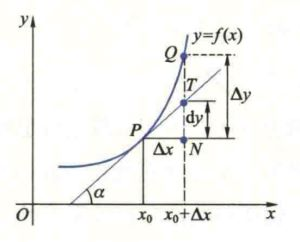
\includegraphics[width=\marginparwidth]{figures/导数的几何意义}
	\caption{导数的几何意义}
	\label{fig:3.1}
\end{marginfigure}

\subsection{从几何意义上}

由\textbf{前面所学的}导数的几何意义,如图\ref{fig:3.1}所示:

我们知道有:当$PN$趋近无穷小的时候,$TN\approx QN$,因此又由$\tan\alpha=f'(x_0)$,故有$f(x)\approx f(x_0)+f'(x_0)(x-x_0)$,\textbf{即在微小局部,用切线段似代替曲线段}。



\section{微分的概念}

\begin{definition}
	设有函数$f:U(x_0)\rightarrow \mathbb{R}$,若存在$\alpha \Delta x$,使$$f(x+\Delta x)-f(x_0)=\alpha\Delta x+o(\Delta x)$$
	\textbf{则称$f$在$x_0$处可微,$\alpha \Delta x$是其微分,记为$\dd f(x_0)=\alpha\Delta x$}
\end{definition}

\subsubsection{微分与导数的关系}

由$\dv{y}{x} = f'(x)$,导数等于函数的微分与之便利的微分之商,因此导数也称为微商。

由式\ref{eq:3.1}的推导,得到:\textbf{可微$\Leftrightarrow$可导}。两个概念互通,所以不区分。

\section{微分的运算、复合与高阶微分}\label{sec:3.3}

\subsection{导数的运算、复合与高阶微分}\label{sec:3.3.1}

请读者自行参考第 \ref{ch:2} 章的内容。

\subsection{微分的运算、复合与高阶微分}\label{sec:3.3.2}
由导数与微分的关系,可以得到
\begin{align*}
	&\dd (u\pm v)=du\pm dv\\
	&\dd(uv)=vdu+udv\\
	&\dd\qty(\frac{u}{v}) = \frac{v\dd u-u\dd v}{v^2}
\end{align*}

设有可微函数$y=f(u)$,而$u$又是另一个变量$x$的可微函数$u=g(x)$,那么复合函数$y=f(g(x))$的微分为

\begin{equation}
	\dd y = f'(u)g'(x)\dd x \label{eq:3.3}
\end{equation}

而我们知道$g'(x)\dd x = \dd u$,故上式可以写为
\begin{equation}
	\dd y = f'(u)\dd u \label{eq:3.4}
\end{equation}

这一性质称为\textbf{微分形式不变性}。

高阶微分,顾名思义就是对一阶微分再求一阶微分,即
\begin{equation*}
	\dd (\dd y) = \dd(f'(x)\dd x) = f''(x)(\dd x)^2
\end{equation*}
也即
\begin{equation}
	\dd^2 f = \dd^2 y = f''(x)\dd x^2\label{eq:3.5}
\end{equation}
对$n$阶微分
\begin{equation}
	\dd^n y = \dd^n f = f^{(n)}\dd x^n\label{eq:3.6}
\end{equation}

\section{微分在近似计算中的应用}\label{sec:3.4}
我们前面说到,微分是在微小局部中用线性主部代替主体的一种思想,那么当我们遇到某些难于计算却存在\textbf{与常见数值只差一个微小局部的计算题}时,我们就可以采用微分进行近似计算,即
\begin{equation}
	f(x+\Delta x)\approx f(x_0)+\alpha\Delta x\label{eq:3.7}
\end{equation}

常用的包括以下近似:
\begin{align*}
	&e^x\approx 1+x\\
	&\sin x\approx x\\
	&\tan x\approx x\\
	&(1+x)^{\alpha}\approx 1+\alpha x\\
	&\ln(1+x)\approx x
\end{align*}

\begin{example}
	计算$\sin44^{\degree}$的近似值\mn{此题是直接存在微小局部,当微小局部没有直接表现出来的时候,要划出微小局部出来。}。
	
	由$\sin(x)=sin(x_0)+(x-x_0)\cos(x_0)$
	
	因为$x_0=\frac{\pi}{4},1^{\degree}=\frac{\pi}{180}$,所以
	$$
	\sin 44^{\degree}\approx\frac{\sqrt{2}}{2}-\frac{\pi}{180}\cos\frac{\rm \pi}{4}\approx 0.6498
	$$
\end{example}

\begin{example}
	计算$\sqrt[5]{270}$的近似值。
	
	当微小局部没有直接表现出来的时候,要划出微小局部出来。
	
	$$
	\sqrt[5]{270}=\sqrt[5]{243+27}=3\qty(1+\frac{27}{243})^{\frac{1}{5}}=3\qty(1+\frac{1}{5}\cdot \frac{27}{243})\approx 3.0667
	$$
\end{example}

\section{模型、套路、题型}
本节没有什么特别要强调的题型,把课后习题做做就好,请各位同学按照老师的要求认真完成作业。